\documentclass[border=10pt]{standalone}
\usepackage{pgfplots}
\usepgfplotslibrary{colormaps}
\pgfplotsset{trig format plots=rad}
\begin{document}
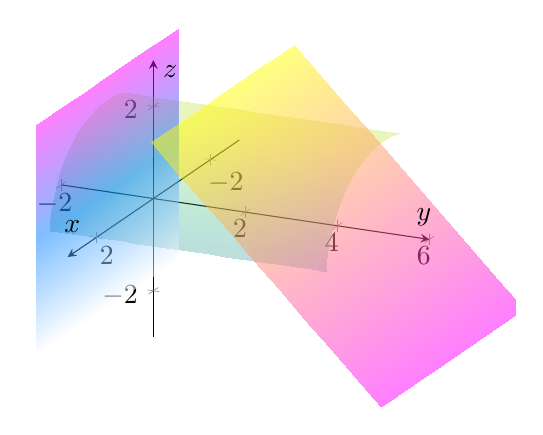
\begin{tikzpicture}
\begin{axis}[
    view={115}{25},
    xlabel=$x$, ylabel=$y$, zlabel=$z$,
    xmin=-3, xmax=3,
    ymin=-2, ymax=6,
    zmin=-3, zmax=3,
    axis lines=center,
    grid=major,
]
% Cylinder x^2 + z^2 = 4
% We use parametric equations for a cylinder.
% x = 2*cos(theta), z = 2*sin(theta)
% y varies from -1 to 4 - z
\addplot3[surf, opacity=0.3, domain=0:2*pi, y domain=-1:5, samples=20, shader=interp, colormap/viridis] 
({2*cos(deg(x))}, {y}, {2*sin(deg(x))});

% Plane 1: y = -1
% We can represent this as a surface with x and z as parameters.
% x = u, z = v, y = -1
\addplot3[surf, opacity=0.5, domain=-2.5:2.5, y domain=-2.5:2.5, samples=10, shader=interp, colormap/cool] 
({x}, {-1}, {y});

% Plane 2: y + z = 4 => y = 4 - z
% x = u, z = v, y = 4 - v
\addplot3[surf, opacity=0.5, domain=-2.5:2.5, y domain=-2.5:2.5, samples=10, shader=interp, colormap/spring] 
({x}, {4-y}, {y});

\end{axis}
\end{tikzpicture}
\end{document}
